\documentclass[xcolor=dvipsnames,beamer]{beamer} %handout,notes=show

\usepackage{textcomp}
\usepackage[utf8]{inputenc}
% \usepackage{default}
\usepackage{graphicx}
%  \usepackage[pdftex]{hyperref}
\usepackage{url}


% frames have to be fragile
\newif\ifnotes
% \notestrue

%\notestrue


\ifnotes
%\setbeamertemplate{note page}[plain]
\setbeamertemplate{note page}[compress]
\setbeamerfont{note page}{size=\large}
\setbeameroption{show only notes}
%\setbeameroption{show notes}
\usepackage{pgfpages}
\pgfpagesuselayout{2 on 1}[a4paper,border shrink=5mm]%
\else
%\setbeameroption{hide notes}
\fi
%\notesfalse



% nastaveni TypeWriter
%\usepackage{courier}
%\usepackage{lmodern}
%\renewcommand*\ttdefault{txtt}
\DeclareFontShape{OT1}{cmtt}{bx}{n}{<5><6><7><8><9><10><10.95><12><14.4><17.28><20.74><24.88>cmttb10}{}


% \usepackage{verbatim}
\usepackage[absolute,overlay]{textpos}

\usepackage{listings}
% \usepackage{courier}
\definecolor{grey}{RGB}{70,70,70}
\definecolor{green}{RGB}{0,255,0}
\definecolor{red}{RGB}{202,53,53}
\definecolor{lightGrey}{RGB}{250,250,250}
\definecolor{darkGrey}{RGB}{50,50,50}


\usepackage{color}
\definecolor{lightgray}{rgb}{.9,.9,.9}
\definecolor{darkgray}{rgb}{.4,.4,.4}
\definecolor{purple}{rgb}{0.65, 0.12, 0.82}


% \usetheme{Warsaw}
\usetheme{Madrid}
% \useoutertheme{infolines}
\usecolortheme[named=MidnightBlue]{structure}
% \usecolortheme[named=PineGreen]{structure}
% \setbeamertemplate{navigation symbols}{}




\title[GRASS GIS 7]
{Image Processing in GRASS GIS 7}
%\subtitle{SVO\v{C}}
%\pdforstring{}{}

\author[Yann Chemin]
{Yann Chemin}

\institute[IWMI]
{International Water Management Institute\\
\vspace{20pt}
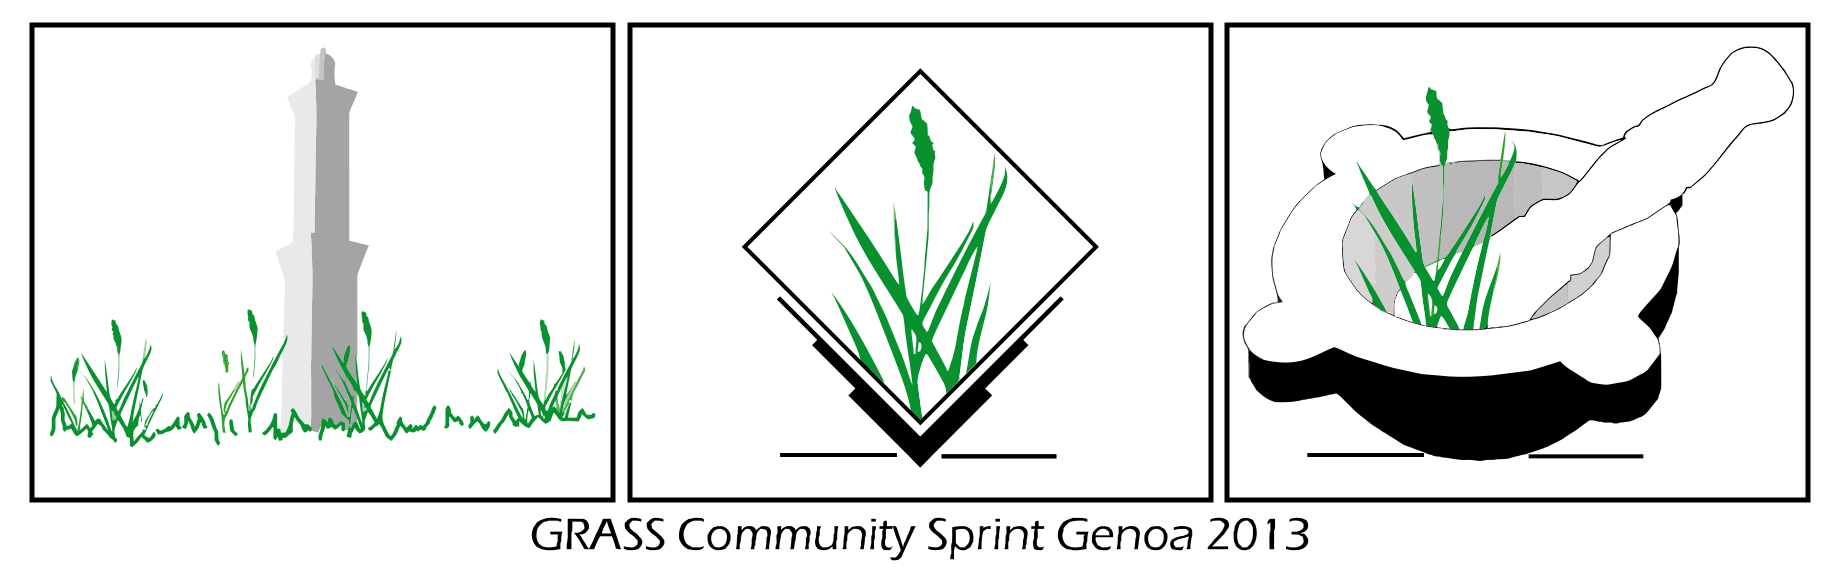
\includegraphics[width=10cm]{genova2013}
}


\date{February 8, 2013}


%\AtBeginSection[]{\begin{frame}\frametitle{Obsah}%
%\tableofcontents[currentsection ]\end{frame}}
%\AtBeginSubsection[]
%{
%  \begin{frame}<beamer>
%  \frametitle{Obsah}
%  \tableofcontents[currentsection,currentsubsection]
%  \end{frame}
%}

\setbeamercovered{transparent}

\hypersetup{%
	pdfauthor={Yann Chemin},%
	pdfsubject={Presentation},%
    pdfkeywords={GRASS, GIS, programming, C}
}

\usepackage{listings}
\lstdefinestyle{C++}{%
  % language
  language=C++, % [ANSI]C++, GNU, ISO, Visual
  basicstyle=\ttfamily\small,
  commentstyle=\itshape,
  keywordstyle=\bfseries, % needs another \ttdefault
  showstringspaces=false,
  stringstyle=,
  identifierstyle=,
  % working with latex
  escapeinside={//lst}{\^^M}  
}

\lstset{%
%  frame=trBL,
%  backgroundcolor=\color{},
  linewidth=\textwidth,
  % working with latex
  gobble=2,
  % float
  nolol=false,
  numberbychapter=true,
  captionpos=t,% tb
  % breaking lines
  breaklines=true,
  breakatwhitespace=true,
  breakindent=10em,
  breakautoindent=true,
  prebreak={},
  postbreak={},
  %document default style
    basicstyle=\ttfamily
}


%\lstlistlistingname % The header name for the list of listings.
%\lstlistingname % The caption label for listings.

\lstnewenvironment{cmdline}[1][]
{\lstset{
  style=C++,
  #1}}
{}

\lstnewenvironment{scpp}[1][]
{\lstset{
  style=C++,
  #1}}
{}

\lstnewenvironment{ncpp}[1][]
{\lstset{
  style=C++,
  numbers=left, 
  numberstyle=\scriptsize, 
  stepnumber=1,
  numbersep=5pt,
  #1}}
{}

\lstnewenvironment{fcpp}[1][]
{\lstset{
  style=C++,
  float,
   % line numbers
  numbers=left, 
  numberstyle=\scriptsize, 
  stepnumber=1,
  numbersep=5pt,
  #1}}
{}


\lstnewenvironment{lcpp}[1][]
{\lstset{%
style=C++,
numbers=left, 
numberstyle=\scriptsize, 
stepnumber=1,
numbersep=5pt,
xleftmargin=12pt,
breakautoindent=false,
breaklines=false,%
#1}}{}

\lstnewenvironment{smallcpp}[1][]
{\lstset{%
style=C++,
numbers=left, 
numberstyle=\tiny, 
stepnumber=1,
numbersep=5pt,
xleftmargin=12pt,
breakautoindent=false,
breaklines=false,%
basicstyle=\ttfamily\scriptsize,
#1}}{}


\lstnewenvironment{pscpp}[1][]
{\lstset{%
style=C++,
xleftmargin=12pt,
breakautoindent=false,
breaklines=false,
#1}}{}


%\lstset{index={square},index={[2]root}}


\newcommand{\overovaciref}[1]{{\scriptsize(\ref{#1})}}


\usepackage{tipa}
\newcommand{\pron}[2]{#1 [#2]}

%%%%%%%%%%%%%%%%%%%%%%%%%%%%%%%%%%%%%%%%%%%%%%%%%%%%%%%%%%%%%%%%%%%%
%%%%%%%%%%%%%%%%%%%%%%%%%%%%%%%%%%%%%%%%%%%%%%%%%%%%%%%%%%%%%%%%%%%%
%%%%%%%%%%%%%%%%%%%%%%%%%%%%%%%%%%%%%%%%%%%%%%%%%%%%%%%%%%%%%%%%%%%%
%%%%%%%%%%%%%%%%%%%%%%%%%%%%%%%%%%%%%%%%%%%%%%%%%%%%%%%%%%%%%%%%%%%%
\begin{document}
%%%%%%%%%%%%%%%%%%%%%%%%%%%%%%%%%%%%%%%%%%%%%%%%%%%%%%%%%%%%%%%%%%%%
\frame{
\titlepage
}
%%%%%%%%%%%%%%%%%%%%%%%%%%%%%%%%%%%%%%%%%%%%%%%%%%%%%%%%%%%%%%%%%%%%%
\begin{frame}{Contents}
\tableofcontents
\end{frame}
%%%%%%%%%%%%%%%%%%%%%%%%%%%%%%%%%%%%%%%%%%%%%%%%%%%%%%%%%%%%%%%%%%%%

\section{Introduction}
\subsection{Overview}
%%%%%%%%%%%%%%%%%%%%%%%%%%%%%%%%%%%%%%%%%%%%%%%%%%%%%%%%%%%%%%%%%%%%
\begin{frame}[fragile]{Overview}

Remote Sensing has been a limited topic in GRASS
\newline\linebreak

\begin{itemize}
 \item GRASS 5: Raw images (esp. aerial photos)
 \item 1990s Public: AVHRR (1100x1100m)
 \item 2000s Public: MODIS (250x250m)
 \item 2010s Public: Landsat (30x30m)
\end{itemize}

Rekindled strong interest from the geospatial community.
\end{frame}

\subsection{Imagery}
%%%%%%%%%%%%%%%%%%%%%%%%%%%%%%%%%%%%%%%%%%%%%%%%%%%%%%%%%%%%%%%%%%%%
\begin{frame}[fragile]{Imagery Functionality}

Remote sensing preparation and product generation\\
Increased interest in the recent years.\\
\bigskip
\begin{itemize}
    \item GRASS 6 (stable) has 33 imagery modules
    \item GRASS 7 (experimental) has 46 modules + 1
    \item Add-ons incubating (many!)
\end{itemize}
\bigskip
Modules also have development stages, \\
from experimental (add-ons) to stable (main).
\newline\linebreak
% From Grass 6 (stable) to Grass 7 (experimental).

GRASS 7 has new temporal and spatial analysis algorithms.

\end{frame}

\subsection{Fundamental developments}
%%%%%%%%%%%%%%%%%%%%%%%%%%%%%%%%%%%%%%%%%%%%%%%%%%%%%%%%%%%%%%%%%%%%
\begin{frame}[fragile]{Imagery developments}

Remanufacturing, performance improvement.\\

\begin{itemize}
 \item i.ortho.photo rewritten (main)
 \item i.atcorr increased speed (main)
 \item i.atcorr more satellite configured (main)
 \item i.pca backward modeling implemented (main) 
\end{itemize}

Preparing Landsat, Aster and MODIS datasets.\\

\begin{itemize}
 \item i.landsat.toar (main), TOA reflectance correction
 \item i.aster.toar (main), TOA reflectance correction
 \item i.modis.qc (main), Quality flag interpretation
\end{itemize}


\end{frame}

%%%%%%%%%%%%%%%%%%%%%%%%%%%%%%%%%%%%%%%%%%%%%%%%%%%%%%%%%%%%%%%%%%%%
\begin{frame}[fragile]{Imagery developments}
Geographical and astronomic functions:\\

\begin{itemize}
 \item i.latlong (main), maps latitude or longitude (dd.ddd)
 \item i.sunhours (main), maps diurnal hours.
\end{itemize}

RS products:\\

\begin{itemize}
 \item i.vi (main), 14 vegetation indices from literature + 1
 \item i.albedo (main), Broadband Albedo (snow \~= 0.6-0.8, water=0.05)
 \item i.emissivity (main), Long wavelength $\lambda$
 \item i.biomass (main), biomass growth for crop yield
\end{itemize}


\end{frame}

%%%%%%%%%%%%%%%%%%%%%%%%%%%%%%%%%%%%%%%%%%%%%%%%%%%%%%%%%%%%%%%%%%%%
\section{Feature identification/classification}
\subsection{Harmonic analysis}
%%%%%%%%%%%%%%%%%%%%%%%%%%%%%%%%%%%%%%%%%%%%%%%%%%%%%%%%%%%%%%%%%%%%
\begin{frame}[fragile]{Harmonic analysis}

Harmonic analysis through incomplete returned Fourier inversion.\\
Only long temporal wavelength return, r.hants (add-ons)\\
Local Maximum Fitting with Akaike Info Content, i.lmf (add-ons)\\

\begin{center}
 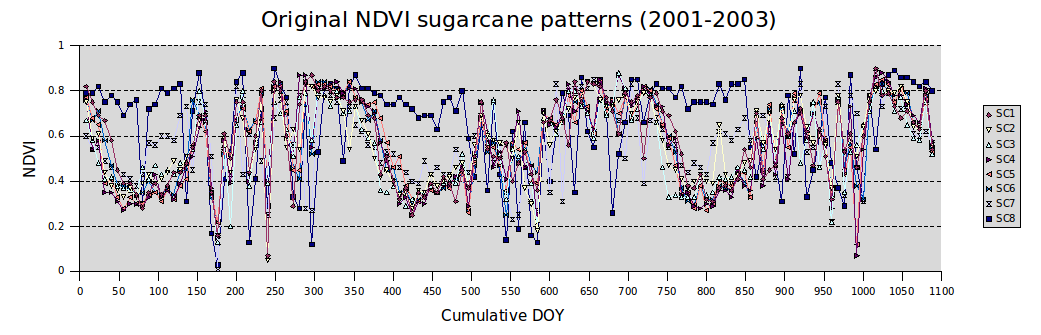
\includegraphics[width=8cm]{hants0}
 \hspace{10mm}
 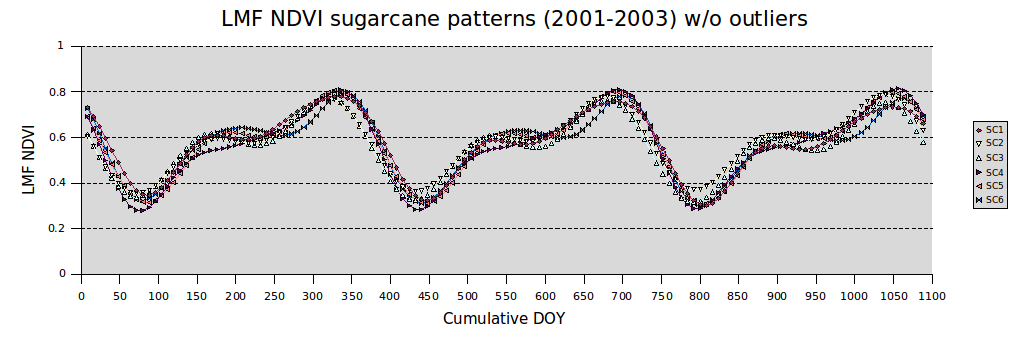
\includegraphics[width=8cm]{hants1}
\end{center}

\end{frame}

\subsection{Segmentation}
%%%%%%%%%%%%%%%%%%%%%%%%%%%%%%%%%%%%%%%%%%%%%%%%%%%%%%%%%%%%%%%%%%%%
\begin{frame}[fragile]{Object recognition}

Segmentation of imagery by object based hierarchical tree classification, i.segment (main)

\begin{center}
 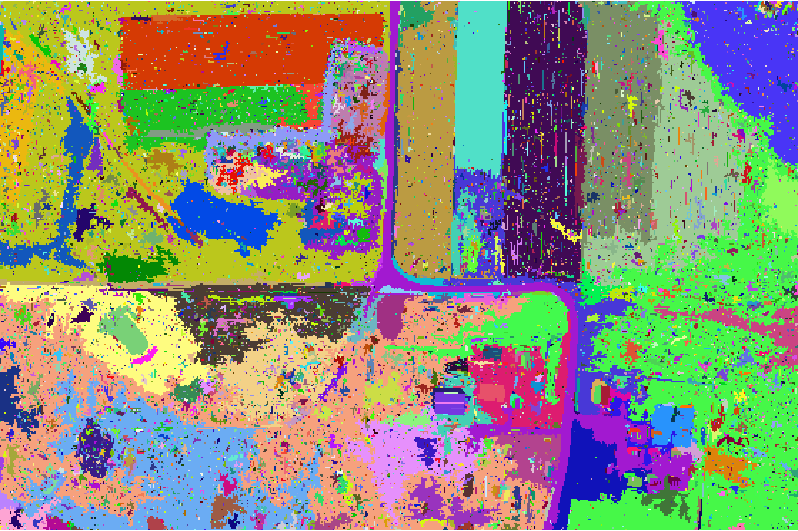
\includegraphics[width=7cm]{i_segment}
\end{center}

\end{frame}

\subsection{Canny}
%%%%%%%%%%%%%%%%%%%%%%%%%%%%%%%%%%%%%%%%%%%%%%%%%%%%%%%%%%%%%%%%%%%%
\begin{frame}[fragile]{Canny}

Edge detection by Canny filter (i.edge in add-ons)\\
Linear features extraction
\begin{center}
 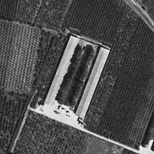
\includegraphics[width=5cm]{farm}
 \hspace{10mm}
 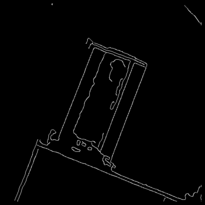
\includegraphics[width=5cm]{farm_canny}
\end{center}

\end{frame}

\section{RS Modeling}
\subsection{Evapotranspiration}
%%%%%%%%%%%%%%%%%%%%%%%%%%%%%%%%%%%%%%%%%%%%%%%%%%%%%%%%%%%%%%%%%%%%
\begin{frame}[fragile]{Evapotranspiration}

Reference/Potential ET: i.evapo.* modules (main)\\

\begin{itemize}
 \item ETo Hargreaves 
 \item ETo Penman-Monteith
 \item ETpot Priestley-Taylor
\end{itemize}

Actual ET: i.eb.* modules (main) using thermodynamic heat flux modeling,\\

\begin{equation}\label{eq1}
\Lambda = \frac {Rn - G - H} {Rn - G}
\end{equation}

\begin{equation}\label{eq2}
ET_a = \Lambda \, ET_{potential}
\end{equation}
\end{frame}

%%%%%%%%%%%%%%%%%%%%%%%%%%%%%%%%%%%%%%%%%%%%%%%%%%%%%%%%%%%%%%%%%%%%
\begin{frame}[fragile]{Evapotranspiration}

Actual evapotranspiration for water/agriculture monitoring and management.\\

\begin{center}
 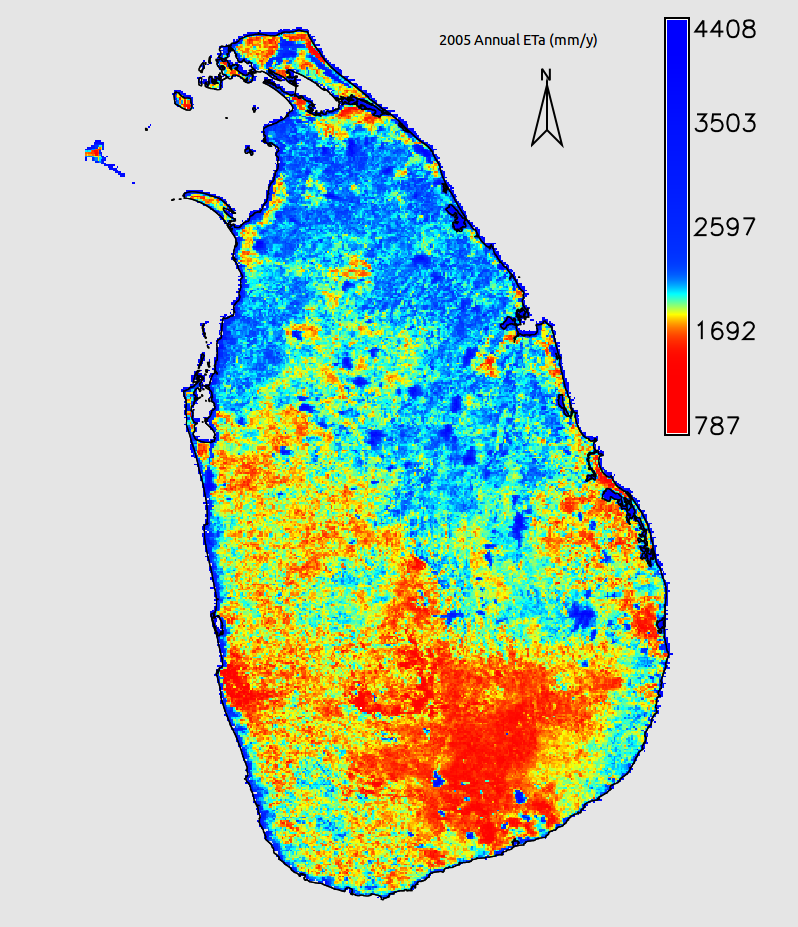
\includegraphics[width=5cm]{slet2005}
 \hspace{10mm}
 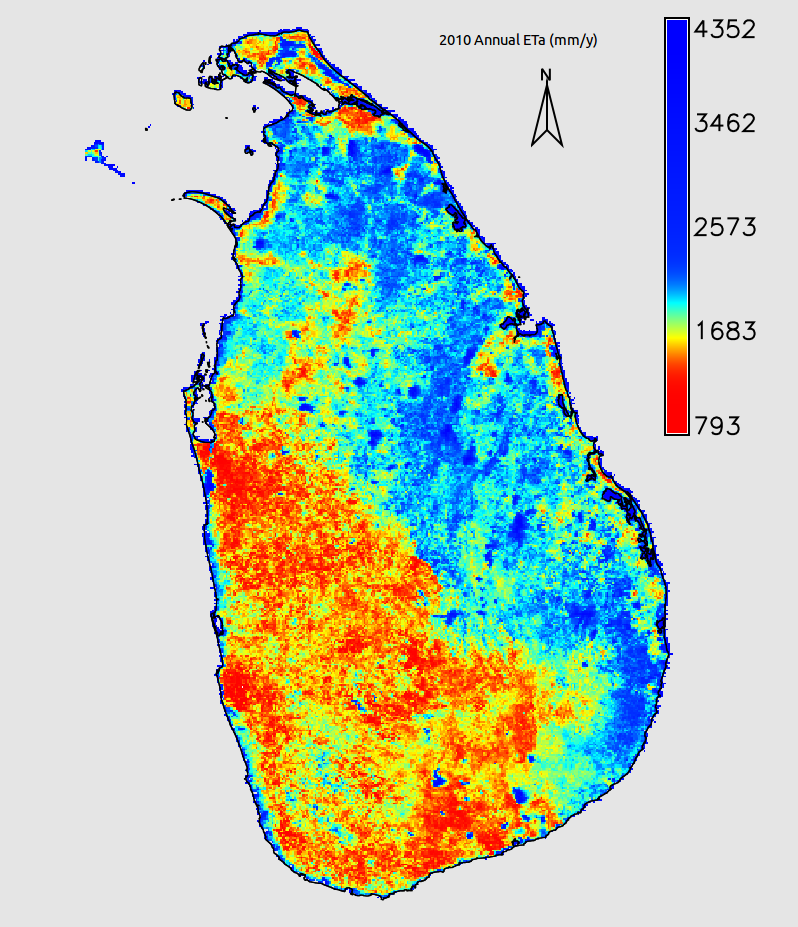
\includegraphics[width=5cm]{slet2010}
\end{center}

\end{frame}

\subsection{Water mapping}
%%%%%%%%%%%%%%%%%%%%%%%%%%%%%%%%%%%%%%%%%%%%%%%%%%%%%%%%%%%%%%%%%%%%
\begin{frame}[fragile]{Water mapping}

Repetitive open water mapping (i.wi, add-ons).\\
Probability of flood destruction on rice crop area in Thailand.

\begin{center}
 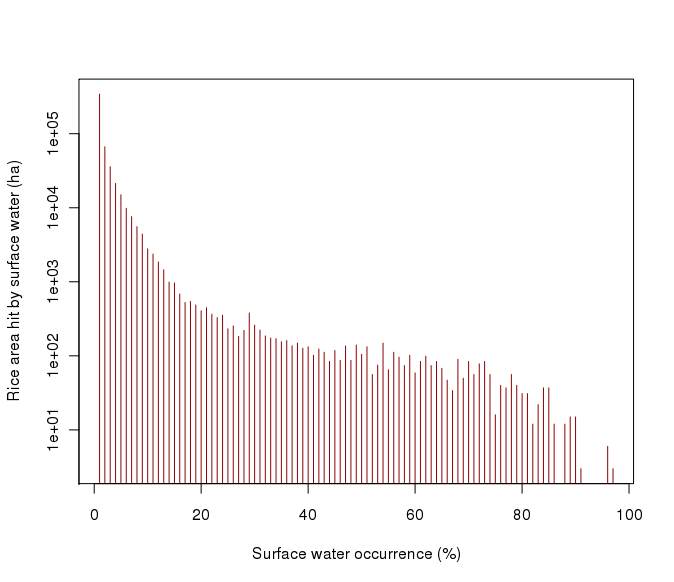
\includegraphics[width=3cm]{flood0}
 \hspace{10mm}
 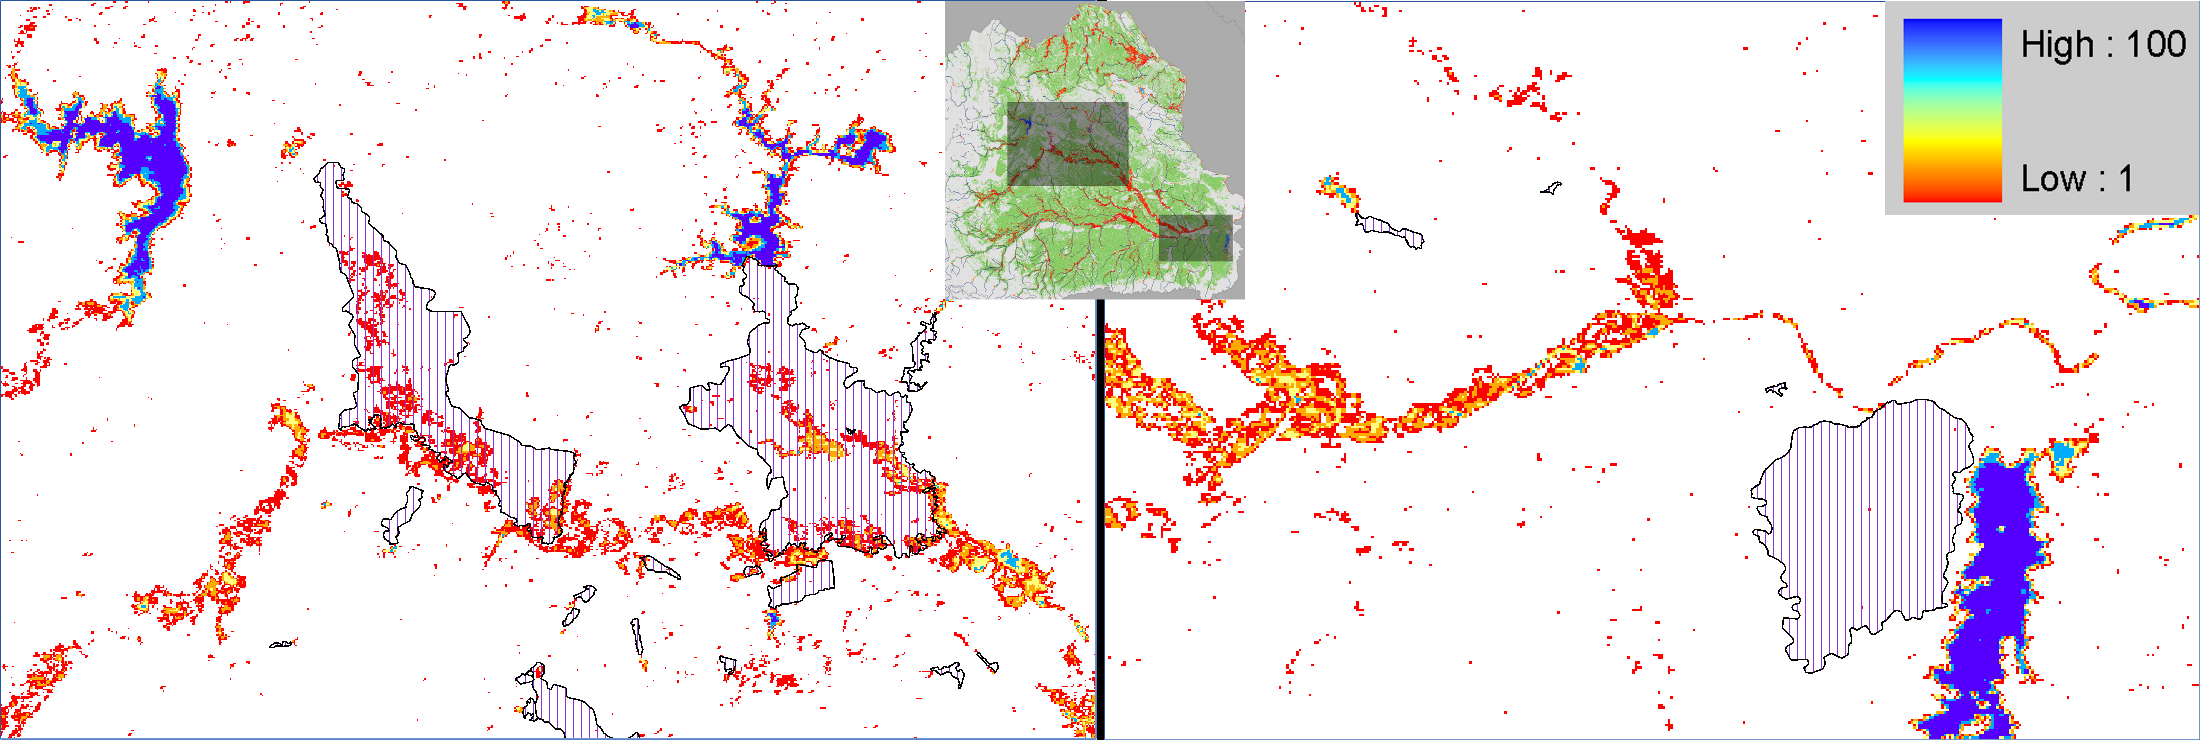
\includegraphics[width=7.5cm]{flood1}
\end{center}

\end{frame}

\subsection{Lidar}
%%%%%%%%%%%%%%%%%%%%%%%%%%%%%%%%%%%%%%%%%%%%%%%%%%%%%%%%%%%%%%%%%%%%
\begin{frame}[fragile]{Lidar}

Lidar reading library permits import into GRASS.\\
On-Farm-Water-Storage Lidar survey and Depth-Volume-Area surveying.

\begin{center}
 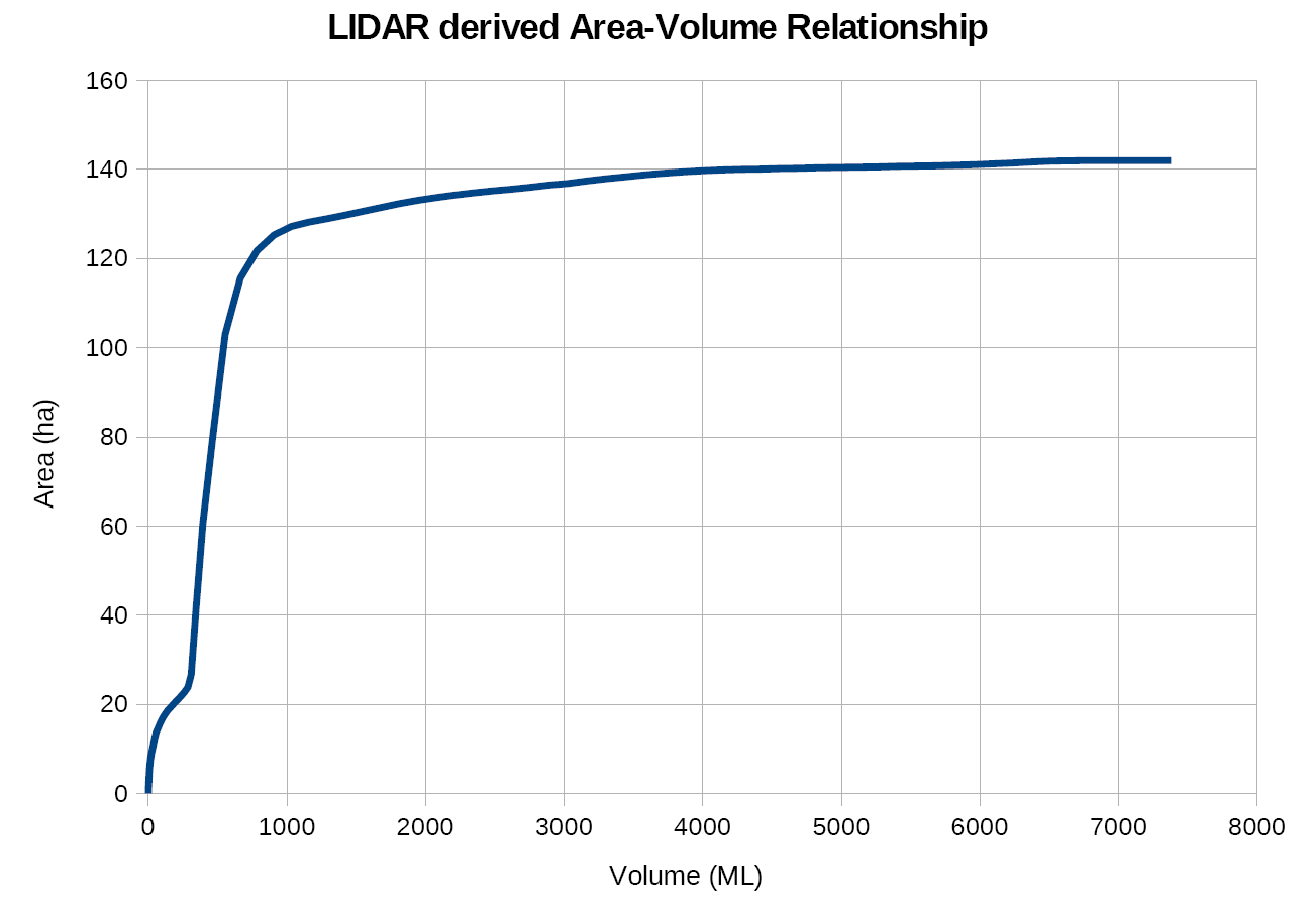
\includegraphics[width=5.5cm]{ofs1}
 \hspace{10mm}
 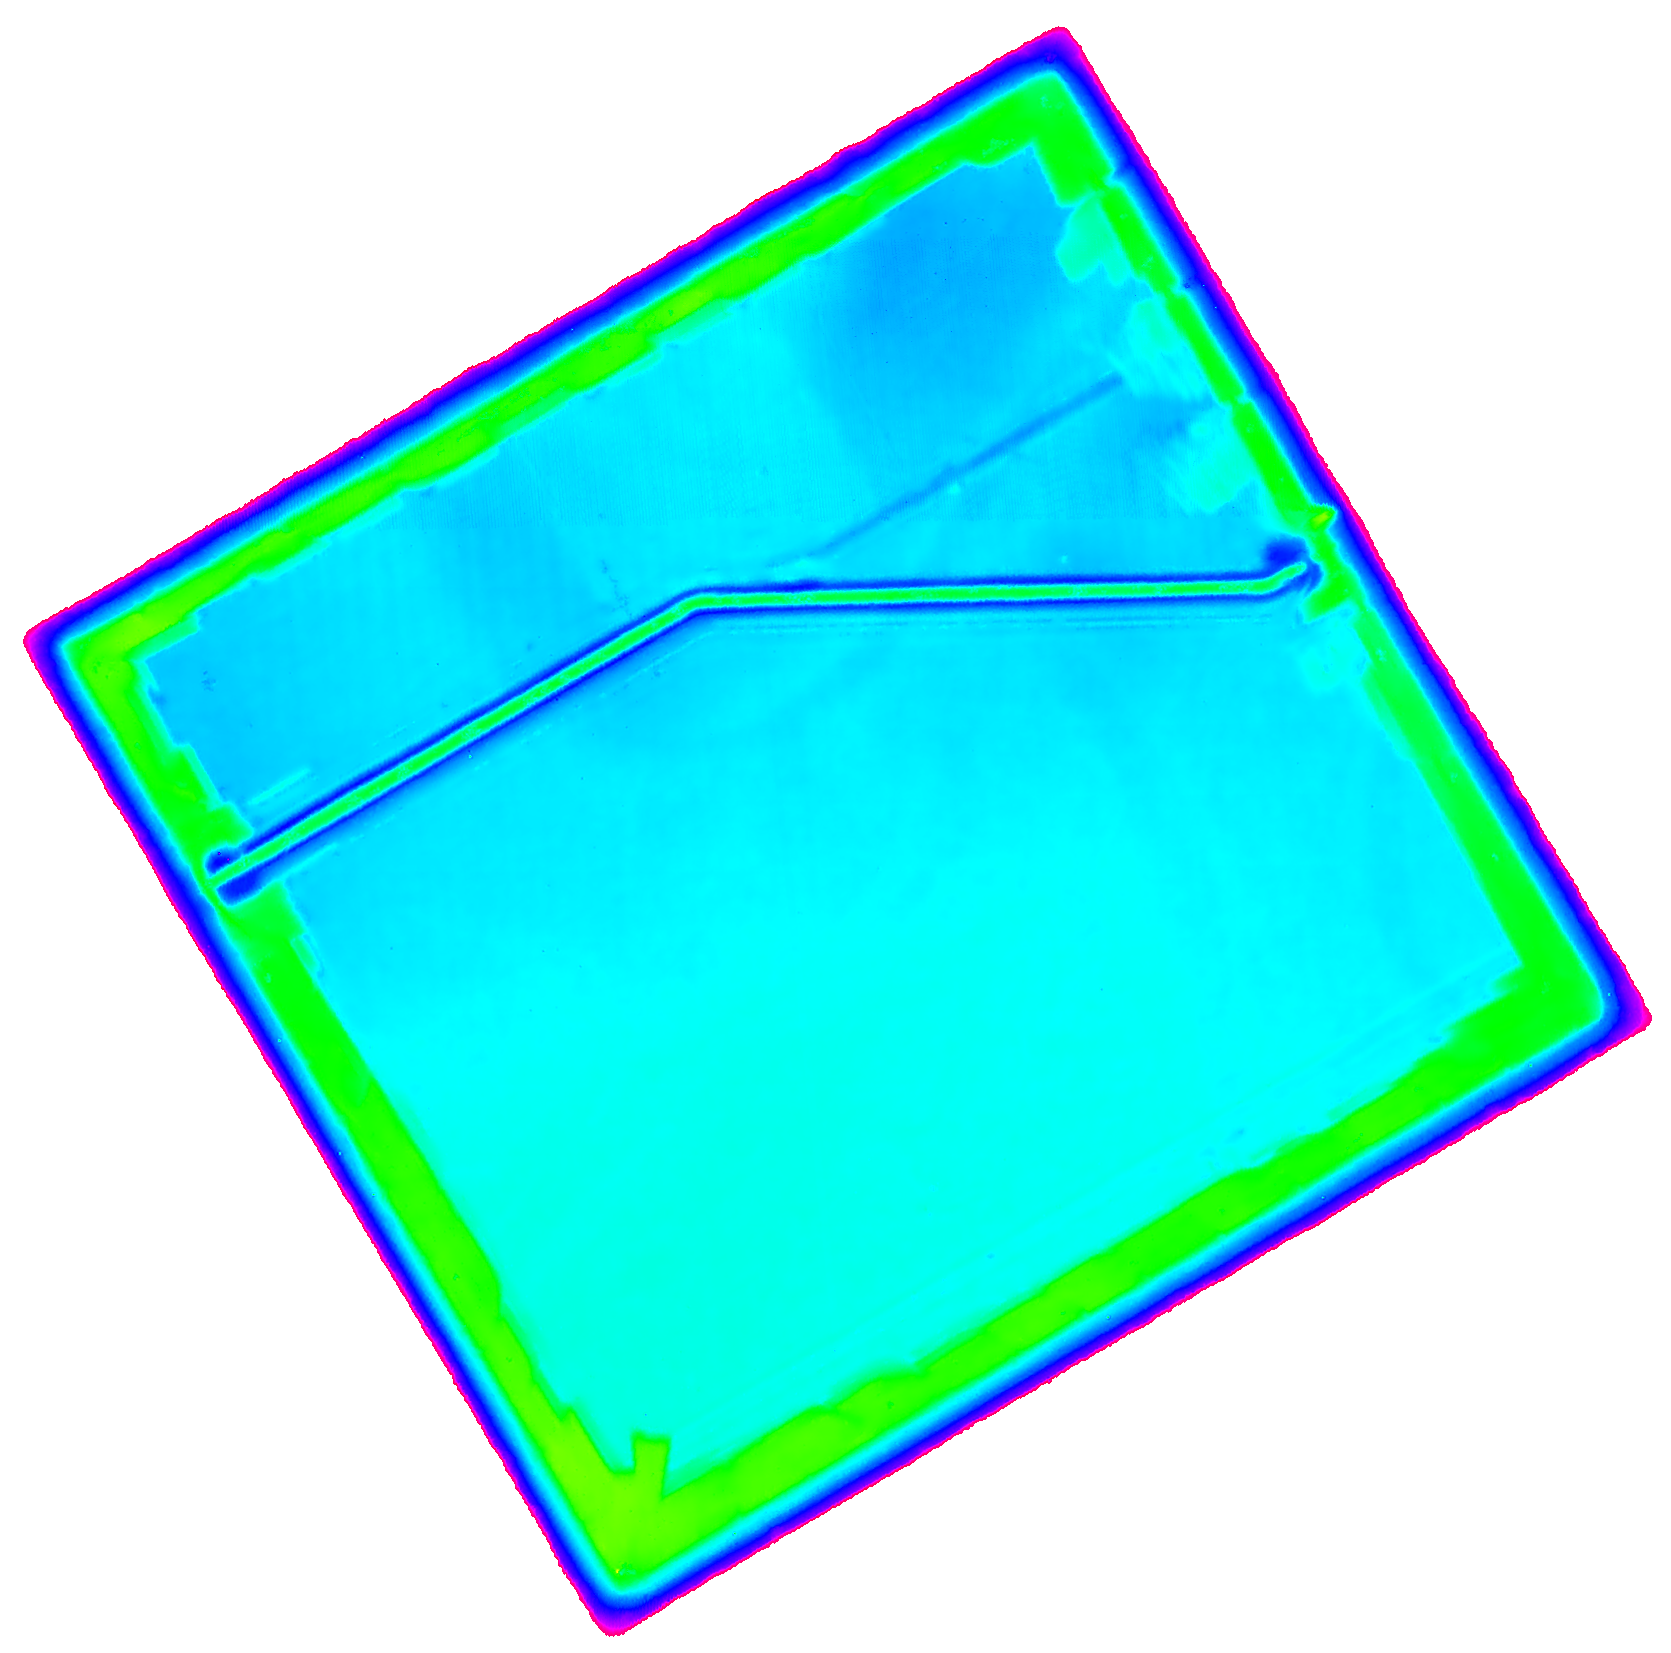
\includegraphics[width=5cm]{ofs2}
\end{center}

\end{frame}

\subsection{Chain processing}
%%%%%%%%%%%%%%%%%%%%%%%%%%%%%%%%%%%%%%%%%%%%%%%%%%%%%%%%%%%%%%%%%%%%
\begin{frame}[fragile]{Chain processing}

Chain processing has a fundamental impact on remote sensing work:\\

\begin{itemize}
 \item Standardization limits bugs
 \item Less prone to human error
 \item Simpler parameterization access
 \item Permits to apply any number of modules to all target images
 \item Ensures maximum quality of generated images
\end{itemize}

Concept: META Module

\end{frame}
%%%%%%%%%%%%%%%%%%%%%%%%%%%%%%%%%%%%%%%%%%%%%%%%%%%%%%%%%%%%%%%%%%%%
\begin{frame}[fragile]{Chain processing}

The development of pyGRASS is maturing,\\
Python and pyGRASS combined can generate META Modules.
\newline\linebreak

\begin{center}
 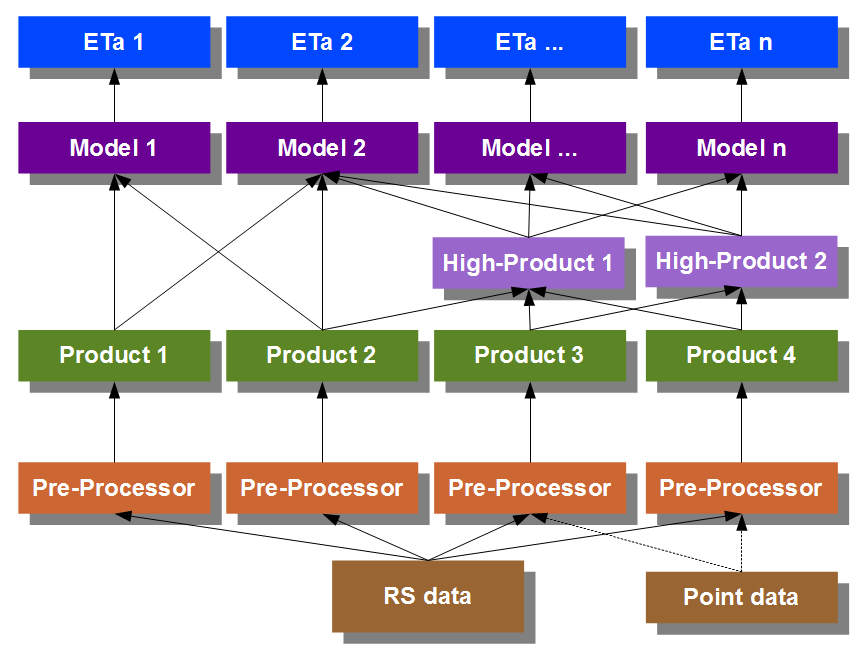
\includegraphics[width=7.5cm]{chain0}
\end{center}

\end{frame}
\section{Other related modules}
%%%%%%%%%%%%%%%%%%%%%%%%%%%%%%%%%%%%%%%%%%%%%%%%%%%%%%%%%%%%%%%%%%%%
\begin{frame}[fragile]{Other related modules}

\begin{itemize}
 \item r.texture (main) for texture based statistic extraction
 \item r.flip (add-ons) for flipping images (i.e. netcdf climate grids)
 \item i.pansharpen (main) for spatial/spectral fusion
 \item i.evapo.* (add-ons) 3 models waiting for integration
 \item i.gravity (add-ons) for GRACE, GOCE, GRAIL (yesterday)
\end{itemize}

\end{frame}
%%%%%%%%%%%%%%%%%%%%%%%%%%%%%%%%%%%%%%%%%%%%%%%%%%%%%%%%%%%%%%%%%%%%
\begin{frame}[fragile]{Thank You}

\begin{center}
 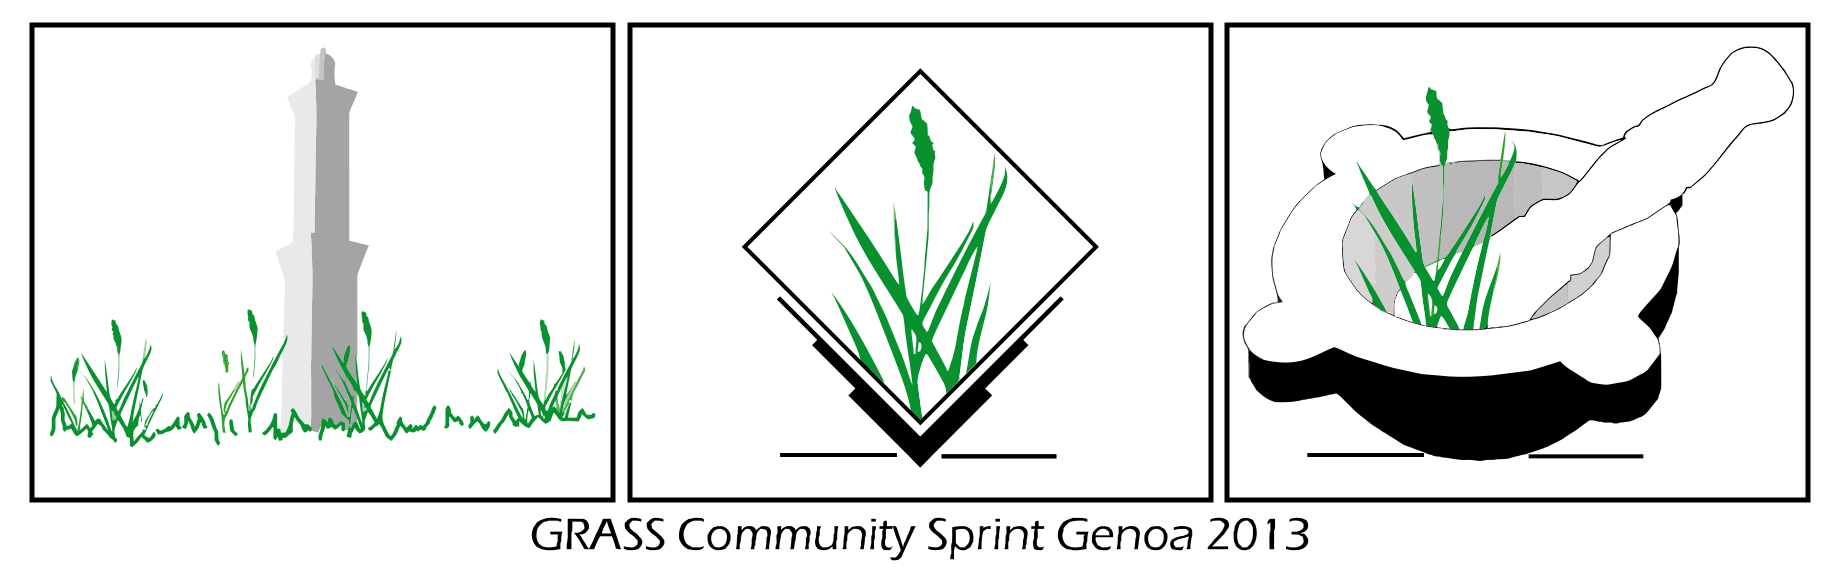
\includegraphics[width=10cm]{genova2013}
\end{center}

\end{frame}

\end{document}
